\documentclass[notes]{subfiles}
\begin{document}
	\addcontentsline{toc}{section}{1.2 - Basic Classes of Functions}
	\setcounter{section}{2}
	\fancyhead[RO,LE]{\bfseries \large \nameref{cs12}} 
	\fancyhead[LO,RE]{\bfseries \currentname}
	\fancyfoot[C]{{}}
	\fancyfoot[LO,RE]{\large \thepage}	%Footer on Right \thepage is pagenumber
	\fancyfoot[RO,LE]{\large Chapter 1.2}

\section*{Classes of Functions}\label{cs12}
	\subsection*{Linear Functions}
		\begin{defn}[Linear Function]
			A \textbf{linear function} takes the form 
			\[f(x) = mx + b\]
			where \(m\) is the slope of the line and \((0,b)\) is the location of the \(y-\)intercept.
		\end{defn}
		
		\begin{defn}[Slope]
			The \textbf{slope} of a line is the ratio of change in output value when the input changes by a specific amount. Given points \((x_1,y_1)\) and \((x_2,y_2)\) on a line, slope is found by
			\[m = \dfrac{y_2-y_1}{x_2-x_1} = \dfrac{\Delta y}{\Delta x}\]
			If we write \(y_1 = f(x_1)\) and \(y_2 = f(x_2)\), then we can write slope as
			\[m = \dfrac{f(x_2)-f(x_1)}{x_2-x_1} = \dfrac{\Delta y}{\Delta x}\]
		\end{defn}
		
		\begin{rmk}[Three Forms of a Line]
			A line is in \textbf{slope-intercept form} if it is written as
			\[y = mx + b\]
			where \(m\) is the slope of the line and \((0,b)\) is the location of the \(y-\)intercept. It is in \textbf{point-slope form} if it is written as
			\[y-y_1 = m(x-x_1)\]
			where \(m\) is the slope of the line and the line goes through the point \((x_1,y_1)\). The line is in \textbf{standard form} if it is written as
			\[ax + by = c\]
			where \(a,b,c\) are real numbers such that \(a,b\) are not both zero.
		\end{rmk}
		
		\begin{rmk}[Four Types of Lines]
			Consider a line of the form \(ax + by = c\).
			\begin{itemize}
				\item If \(a,b \neq 0\), then the line has slope \(m = -\dfrac{a}{b}\) and passes through the point \(\lrpar{0,\dfrac{c}{b}}\). In particular, it is neither horizontal nor vertical.
				\item If \(a = 0\), then the line has slope \(m = 0\) and passes through the point \(\lrpar{0,\dfrac{c}{b}}\). In particular, it is horizontal with equation \(y = \dfrac{c}{b}\).
				\item If \(b = 0\), then the line has undefined slope and passes through the point \(\lrpar{\dfrac{c}{a},0}\). In particular, it is vertical with equation \(x = \dfrac{c}{a}\).
			\end{itemize}
		\end{rmk}
		
	\subsection*{Polynomial Functions}
		\begin{defn}[Polynomial Function]
			A function \(f(x)\) is called a \textbf{polynomial} if it takes the form
				\[P(x) = a_nx^n + a_{n-1}x^{n-1} + \cdots + a_2x^2 + a_1x + a_0\]
			where \(n\) is a nonnegative integer and the numbers \(a_i\) are called the \emph{coefficients} of the polynomial. The \emph{degree} of the polynomial is the power of the leading term, \(n\).
		\end{defn}
		
		Polynomials have nice domain and range, as shown below. Here, \(k\) is some real number (which depends on the function):
	 	\begin{center}
	 		\setlength{\arrayrulewidth}{1.5pt}
	 		\renewcommand{\arraystretch}{1.5}
	 		\begin{tabular}{|c|c|c|}\hline
	 			\multicolumn{3}{|c|}{{\large \textbf{Properties of Polynomials}}} \\ \hline
	 			
	 			& \textbf{Domain} & \textbf{Range} \\ \hline
	 			\textbf{Even Degree}, \(a_n > 0\) & \((-\infty,\infty)\) & \((k, \infty)\) \\ \hline
	 			\textbf{Even Degree}, \(a_n < 0\) & \((-\infty,\infty)\) & \((-\infty,k)\) \\ \hline
	 			\textbf{Odd Degree}, \(a_n > 0\) & \((-\infty,\infty)\) & \((-\infty,\infty)\) \\ \hline
	 			\textbf{Odd Degree}, \(a_n < 0\) & \((-\infty,\infty)\) & \((-\infty,\infty)\) \\ \hline
	 		\end{tabular}
	 	\end{center}
	 		\newpage
		
		Some common polynomials are described below:
		\begin{center}
	 		%\tabulinesep = 2mm	 	
	 		\setlength{\arrayrulewidth}{1.5pt}
	 		\renewcommand{\arraystretch}{1.5}	
	 		\begin{tabular}{| c|c | c |c|}\hline 
	 			\multicolumn{4}{|c|}{{\large \textbf{Common Polynomials}}} \\ \hline
	 			
	 			\textbf{Polynomial} 	& \textbf{Equation}	& \textbf{Graph} (\(a_n > 0\))	& \textbf{Graph} (\(a_n < 0\)) \\ \hline 
				Linear				& \(a_1x + a_0\) & 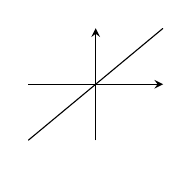
\begin{tikzpicture}\begin{axis}[scale = .25, axis x line = middle, axis y line = middle, ticks = none] \addplot[domain = -1:1] {x}; \end{axis} \end{tikzpicture} & 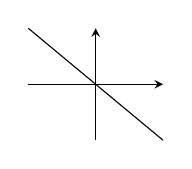
\begin{tikzpicture}\begin{axis}[scale = .25, axis x line = middle, axis y line = middle, ticks = none] \addplot[domain = -1:1] {-1*x}; \end{axis} \end{tikzpicture} \\ \hline
				
				Quadratic			& \(a_2x^2 + a_1x + a_0\)	& 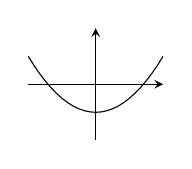
\begin{tikzpicture}\begin{axis}[scale = .25, axis x line = middle, axis y line = middle, ticks = none, ymin = -1, ymax = 1] \addplot[domain = -1:1] {x^2-.5}; \end{axis} \end{tikzpicture} & 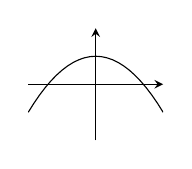
\begin{tikzpicture}\begin{axis}[scale = .25, axis x line = center, axis y line = middle, ticks = none, ymin = -1, ymax = 1] \addplot[domain = -1:1] {-1*x^2 + .5}; \end{axis} \end{tikzpicture} \\ \hline
		 		
		 		Cubic				& \(a_3x^3 + a_2x^2 + a_1x + a_0\)	& 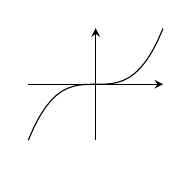
\begin{tikzpicture}\begin{axis}[scale = .25, axis x line = middle, axis y line = middle, ticks = none] \addplot[domain = -1:1] {x^3}; \end{axis} \end{tikzpicture} & 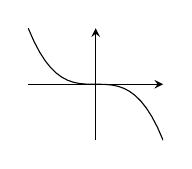
\begin{tikzpicture}\begin{axis}[scale = .25, axis x line = middle, axis y line = middle, ticks = none] \addplot[domain = -1:1] {-1*x^3}; \end{axis} \end{tikzpicture} \\ \hline
		 		
		 		Even Degree			& \makecell{\(a_nx^n + \cdots a_1x + a_0\) \\ \(n\) even}	& \begin{tikzpicture}\begin{axis}[scale = .25, axis x line = middle, axis y line = middle, ticks = none, ymin = -1, ymax = 1] \addplot[<-,domain = -1:-.75] {x^2 -.5}; \addplot[domain = -.75:.75, dotted] {x^2-.5}; \addplot[domain = .75:1,->] {x^2-.5}; \end{axis} \end{tikzpicture} & \begin{tikzpicture}\begin{axis}[scale = .25, axis x line = middle, axis y line = middle, ticks = none, ymin = -1, ymax = 1] \addplot[<-,domain = -1:-.75] {-1*x^2 + .5}; \addplot[domain = -.75:.75, dotted] {-1*x^2 + .5}; \addplot[domain = .75:1,->] {-1*x^2 + .5}; \end{axis} \end{tikzpicture} \\ \hline
		 		
		 		Odd Degree			& \makecell{\(a_nx^n + \cdots a_1x + a_0\) \\ \(n\) odd}	& \begin{tikzpicture}\begin{axis}[scale = .25, axis x line = middle, axis y line = middle, ticks = none] \addplot[<-,domain = -1:-.75] {x^3}; \addplot[domain = -.75:.75, dotted] {x^3}; \addplot[domain = .75:1,->] {x^3}; \end{axis} \end{tikzpicture} & \begin{tikzpicture}\begin{axis}[scale = .25, axis x line = middle, axis y line = middle, ticks = none] \addplot[<-,domain = -1:-.75] {-1*x^3}; \addplot[domain = -.75:.75, dotted] {-1*x^3}; \addplot[domain = .75:1,->] {-1*x^3}; \end{axis} \end{tikzpicture} \\ \hline
		 	\end{tabular}
	 	\end{center}
	 	
	 	\begin{rmk}[Zeros of a Polynomial]
	 		The zeros of any polynomial \(f(x)\) are found by solving the equation
	 			\[f(x) = 0\]
			In particular, if \(f(x)\) has zeros \(x_1,...,x_k\), then \(f(x)\) can be written as
				\[f(x) = (x-x_1)(x-x_2)\cdots (x-x_k)\]
			A zero is said to have \emph{multiplicity} \(n\) if the factor \(x-x_j\) occurs \(n\) times.
	 	\end{rmk}
	 	
	 	\begin{rmk}[Quadratic Formula]
	 		For a quadratic function of the form \(ax^2 + bx + c = 0\), the solutions are given by 
	 			\[x = \dfrac{-b \pm \sqrt{b^2 -4ac}}{2a}\]
			The term \(b^2-4ac\) is called the \emph{discriminant} of the quadratic.
	 	\end{rmk}
	 	
	 	\begin{rmk}[Number of Solutions to a Quadratic]
	 		A quadratic function \(f(x) = ax^2 + bx + c\) has
	 		\begin{itemize}
	 			\item two real solutions if \(b^2-4ac > 0\)
	 			\item one real solution if \(b^2-4ac = 0\)
	 			\item zero real solutions if \(b^2-4ac < 0\)
	 		\end{itemize}
	 		While a quadratic technically has two complex conjugate solutions if the discriminant is negative, we work exclusively with real numbers in the calculus sequence.
	 	\end{rmk}
	 	
	 	\begin{rmk}[Location of the Zeros of a Quadratic]
	 		The \emph{vertex} of a quadratic function is located at the point
	 			\[\lrpar{-\dfrac{b}{2a},f\lrpar{-\dfrac{b}{2a}}}\]
			The zeros, if they exist, are located at 
				\[x = -\dfrac{b}{2a} + \dfrac{\sqrt{b^2-4ac}}{2a}\]
				and
				\[x = -\dfrac{b}{2a} - \dfrac{\sqrt{b^2-4ac}}{2a}\]
			i.e., the zeros are always \(\dfrac{\sqrt{b^2-4ac}}{2a}\) units away from the vertex.
	 	\end{rmk}
	 	\begin{ex}
	 		Consider the quadratic function \(f(x) = 2x^2 -9x -5\). 
	 		\begin{enumerate}[(a)]
	 			\item Use the quadratic formula to identify the zeros of the function.
	 				\vs{1}
	 				\newpage
	 				
				\item Find the zeros again, but this time by factoring.
					\vs{1}
					
				\item What is the range of \(f(x)\)?
					\vs{1}
	 		\end{enumerate}
	 	\end{ex}
	 	
	\subsection*{Rational Functions}
		\begin{defn}[Rational Function]
			A \textbf{rational function} is one which takes the form
				\[f(x) = \dfrac{P(x)}{Q(x)}\]
			where \(P(x),Q(x)\) are polynomials.
		\end{defn}
		
		\begin{rmk}[Domain of Rational Functions]
			The domain of a rational function \(f(x) = \dfrac{P(x)}{Q(x)}\) is the set
				\[\text{Dom}\,(f) = \lrbrace{x \mid Q(x)\neq 0}\]
		\end{rmk}
			\newpage
			
		\begin{rmk}[Graphs of Rationals: Holes vs. Vertical Asymptotes]
			For rational function \(f(x) = \dfrac{P(x)}{Q(x)}\), assume \(P(x)\) can be factored (not counting multiplicity) as
				\[P(x) = (x-x_{p_1})\cdots (x-x_{p_n})\]
			where \(n\) is the degree of the \(P(x)\), and \(Q(x)\) can be factored (not counting multiplicity) as
				\[Q(x) = (x-x_{q_1})\cdots (x-x_{q_k})\]
			where \(k\) is the degree of \(Q(x)\).  Then,
			\begin{itemize}
				\item The graph of \(f(x)\) has vertical asymptote at \(x = x_i\) for every factor \(x-x_i\) which \emph{is not} shared by \(P(x)\) and \(Q(x)\)
				\item The graph of \(f(x)\) has a hole at the input \(x = x_j\) for every factor \(x-x_j\) which \emph{is} shared by \(P(x)\) and \(Q(x)\)
			\end{itemize}
		\end{rmk}
		
		\begin{ex}
			Consider the function \(f(x) = \dfrac{(x-1)(x-2)}{(x-1)^2(x-2)(x+3)}\)
			\begin{enumerate}[(a)]
				\item Identify the domain of \(f(x)\).
					\vs{1}
					
				\item Use part (a) to find any vertical asymptotes in the graph of \(f(x)\).
					\vs{1}
					
				\item \(f(x)\) has one hole in its graph; where is it?
					\vs{1}
					
			\end{enumerate}
		\end{ex}
			\newpage
			
	\subsection*{Power Functions}
		\begin{defn}[Power Function]
			A \textbf{power function} is any function of the form \(f(x) = x^a\), where \(a\) is any real number.
		\end{defn}
		
		\begin{question}
			Describe the difference between a power function of the form \(f(x) = x^a\) and a polynomial of the form \(g(x) = x^b\).
		\end{question}
			\vs{1}
			
		\begin{rmk}[Special Power Functions]
			There are a few power functions which see special use.
			\begin{itemize}
				\item If \(a = \dfrac{1}{n}\), where \(n \geq 2\) is an integer, then we call the function \(f(x) = x^a = x^{1/n}\) a \textbf{root function}, since the rules of exponents say that \(x^{1/n} = \sqrt[n]{x}\). If \(n = 2\), then we have a square root function; if \(n = 3\), we have a cube root function.
				\item If \(a = -1\), then the function \(f(x) = x^{-1} = \dfrac{1}{x}\) is called the \textbf{reciprocal function}. The reciprocal function can also be considered a rational function, with \(P(x) = 1\) and \(Q(x) = x\).
			\end{itemize}
		\end{rmk}
		
		
	\subsection*{Algebraic \& Transcendental Functions}
		\begin{defn}[Algebraic Function]
			The function \(f(x)\) is called \textbf{algebraic} if it can be constructed using algebraic operations such as addition, subtraction, multiplication, division, and taking roots, starting with polynomials.
		\end{defn}
			\newpage
			
		\begin{ex}
			Find the domain of the function \(f(x) = \dfrac{9x^2 -1}{\sqrt{4x + 5}}\)
		\end{ex}
			\vs{1}
			
		\begin{defn}[Exponential/Logarithmic Function]
			An \textbf{exponential function} is a function of the form \(f(x) = b^x\), where the base \(b\) is a positive constant. A \textbf{logarithmic function} is a function of the form \(g(x) = \log_b (x)\), where the base \(b\) is a positive constant.
		\end{defn}
		
		\begin{center}
			\setlength{\arrayrulewidth}{1.5pt}
			\renewcommand{\arraystretch}{1.5}
			\begin{tabular}{|c|c|c|c|}\hline
				\multicolumn{4}{|c|}{\textbf{Properties of Transcendental Functions}}\\ \hline
				\textbf{Function} & \textbf{Domain} & \textbf{Range} & \textbf{Asymptote} \\ \hline
				\(f(x) = b^x\) & \((-\infty,\infty)\) & \((0,\infty)\) & \(y = 0\) \\ \hline
				\(g(x) = \log_b (x)\) & \((0,\infty)\) & \((-\infty,\infty)\) & \(x = 0\) \\ \hline
			\end{tabular}
		\end{center}
		
		\begin{ex}
			Find the domain of the function \(k(r) = \log_5(r^2 -2r+3)\)
		\end{ex}
			\vs{1}
			\newpage
			
	\subsection*{Piecewise Functions}
		\begin{defn}[Piecewise Function]
			A \textbf{piecewise function} is a function defined by different formulas in different parts of their domains.
		\end{defn}
						
		\begin{ex}
			A quick example of a piecewise function is the \emph{absolute value function}: 
				\[f(x) = |x| = \begin{cases}-x & x < 0 \\x & x \geq 0  \end{cases}\]
				
			\begin{enumerate}[(a)]
				\item What is \(f(-5)\)? What about \(f(1)\)?
					\vs{.5}
					
				\item What is \(f(0)\)?  Why?
					\vs{.5}
					
				\item Sketch \(|x|\) on the interval \(-5\leq x \leq 5\).
					\vs{1}
			\end{enumerate}
		\end{ex}
			
		\begin{ex}
			Write the absolute value function \(f(x) = |2x-3|\) as a piecewise function
		\end{ex}
			\vs{1.5}
			\newpage
			
	\subsection*{Transformations of Functions}
		\begin{rmk}[Vertical and Horizontal Shifts]
			Let \(c > 0\).  To obtain the graph of
				\begin{itemize}
					\item \(y = f(x) + c\), shift the graph of \(y = f(x)\) \(c\) units up.
					\item \(y = f(x) - c\), shift the graph of \(y = f(x)\) \(c\) units down.
					\item \(y = f(x+c)\), shift the graph of \(y = f(x)\) \(c\) units left.
					\item \(y = f(x-c)\), shift the graph of \(y = f(x\) \(c\) units right.
				\end{itemize}
		\end{rmk}
		\begin{rmk}[Vertical and Horizontal Stretching/Reflecting]
			Let \(c > 1\).  To obtain the graph of
				\begin{itemize}
					\item \(y = c\cdot f(x)\), stretch the graph of \(y = f(x)\) vertically by a factor of \(c\).
					\item \(y = \lrpar{\dfrac{1}{c}}f(x)\), shrink the graph of \(y = f(x)\) vertically by a factor of \(c\).
					\item \(y = f(c\cdot x)\), shrink the graph of \(y = f(x)\) horizontally by a factor of \(c\).
					\item \(y = f\lrpar{\dfrac{x}{c}}\), stretch the graph of \(y = f(x)\) horizontally by a factor of \(c\).
					\item \(y = -f(x)\), reflect the graph of \(y = f(x)\) about the \(x-\)axis.
					\item \(y = f(-x)\), reflect the graph of \(y = f(x)\) about the \(y-\)axis.
				\end{itemize}
		\end{rmk}
		
		\begin{ex}
			If \(g(1) = 3\), then what point must be on the graph of \(h(t) = -2g(t-1) + 6\)?
		\end{ex}
			\vs{1}
			\newpage
		
		\begin{ex}
				Sketch the graph of the function \(f(x) = x^2 - 2x +3\) by applying transformations to the base graph of \(f(x) = x^2\).
				\begin{center}
				\begin{tabular}{cc}
					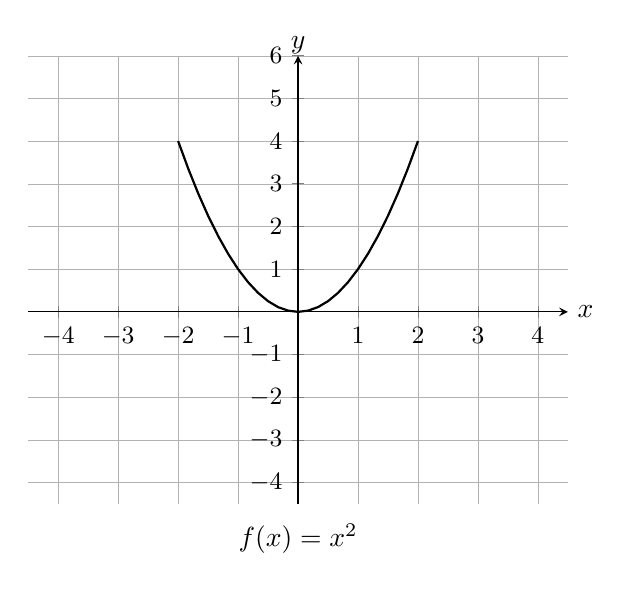
\begin{tikzpicture}
						\begin{axis}[
							grid style = {line width = .1pt, draw = gray!60},
							grid = both,
							every tick label/.append style={font=\small},
							axis x line = middle,
							axis y line = middle,
				    			every axis y label/.style={at={(ticklabel cs:1.15)}, yshift = -3pt},
								y label style={at={(axis description cs: 0.5, 1)},above},
							ytick = {-4,-3,-2,-1,1,2,3,4,5,6},
				    			ylabel = {$y$},
				    			ymin = -4.5, ymax = 6,
			    				every axis x label/.style= {at ={(ticklabel cs:1)}},
			    				xtick = {-4,-3,-2,-1,1,2,3,4},
				    				x label style={at={(axis description cs: 1, 0.43)},right},
			    				xlabel = {$x$},
			    				xmin = -4.5, xmax = 4.5,
						]
							\addplot[thick, domain = -2:2] {x^2};
							\coordinate (label) at (0,-5);
						\end{axis}						
						\draw (label) node[yshift = -5pt] {$f(x) = x^2$};
					\end{tikzpicture}
					&
					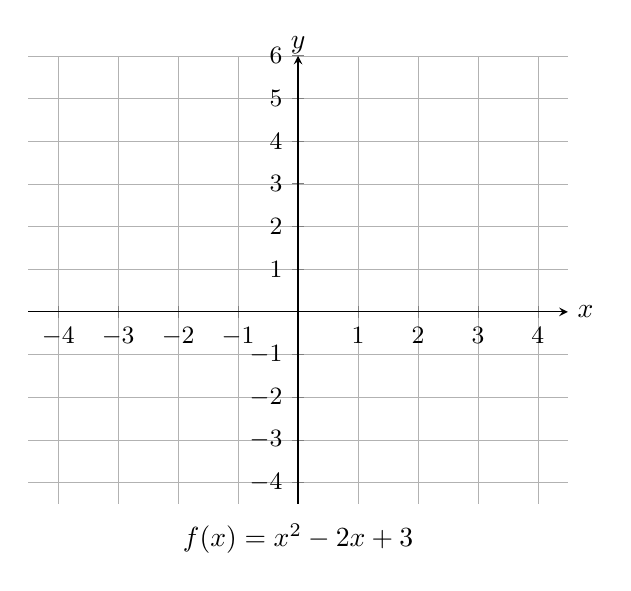
\begin{tikzpicture}
						\begin{axis}[
							grid style = {line width = .1pt, draw = gray!60},
							grid = both,
							every tick label/.append style={font=\small},
							axis x line = middle,
							axis y line = middle,
				    			every axis y label/.style={at={(ticklabel cs:1.15)}, yshift = -3pt},
								y label style={at={(axis description cs: 0.5, 1)},above},
							ytick = {-4,-3,-2,-1,1,2,3,4,5,6},
				    			ylabel = {$y$},
				    			ymin = -4.5, ymax = 6,
			    				every axis x label/.style= {at ={(ticklabel cs:1)}},
			    				xtick = {-4,-3,-2,-1,1,2,3,4},
				    				x label style={at={(axis description cs: 1, 0.43)},right},
			    				xlabel = {$x$},
			    				xmin = -4.5, xmax = 4.5
						]
							\coordinate (label) at (0,-5);
						\end{axis}
						\draw (label) node[yshift = -5pt] {$f(x) = x^2-2x+3$};
					\end{tikzpicture}
				\end{tabular}
				\end{center}
			\end{ex}
				\vs{1}

		\begin{ex}
			Sketch the graphs of the given functions by using transformations to base graph:
			\begin{enumerate}[(a)]
				\item \(f(x) = \dfrac{-2}{x+3}\)
					\vs{1}
					
				\item \(g(x) = 1-\cos 2x\)
					\vs{1}
			\end{enumerate}				
		\end{ex}	

		
				
		
			
		
\clearpage
\end{document}